\documentclass[9pt,twocolumn,twoside]{../../styles/osajnl}

\journal{i524} 

\title{An Overview of Pivotal Web Services}


\author[1,*]{Harshit Krishnakumar}

\affil[1]{School of Informatics and Computing, Bloomington, IN 47408, U.S.A.}
\affil[*]{Corresponding authors: harkrish@iu.edu, S17-IR-2014}

\dates{Project-02, \today}

\ociscodes{Cloud, I524, Web Services}

% replace this with your url in github/gitlab
\doi{\url{https://github.com/cloudmesh/sp17-i524/raw/master/paper2/S17-IR-2014/report.pdf}}


\begin{abstract}
Pivotal Web Services is a platform as a service (PAAS) provider which allows developers to deploy applications written in six different languages. It has options to automatically bind 21 integrated addons to applications, and allows vertical and horizontal scaling \cite{www-paasfinder}. This paper presents the different features of Pivotal Web Services and a basic overview of hands-on of application deployment in Pivotal Web Services.
\newline
\end{abstract}

\setboolean{displaycopyright}{true}

\begin{document}

\maketitle

\TODO{This review document is provided for you to achieve your
  best. We have listed a number of obvious opportunities for
  improvement. When improving it, please keep this copy untouched and
  instead focus on improving report.tex. The review does not include
  all possible improvement suggestions and for each comment you may
  want to check if it applies elsewhere in the document.}

\TODO{Assessment: Some revisions suggested. Please address the review
  comments below.}

\TODO{Abstract: The citations is not necessary here. It should go in
  the main text.}

\TODO{Abstract: That PWS binds 21 addons is minutiae that doesn't
  belong in the abstract.}

\TODO{Abstract: Overall, abstract is on the short side and could do a
  better job of describing what PWS is and its value to someone
  without background in PAAS. Please revisit.}

\TODO{In general: You need to focus your paper a little more on
  PWS. You spend too much on some of the background material that will
  either be familiar to a reader, or should be explained more
  succinctly. At the same time, the actual discussion of PWS is light
  in the paper and should be expanded with examples. Writing a Use
  Case section would go a long way towards making the paper more
  informative. Finally, you have some places where the language is
  subjective or more suited to a press release than a neutral
  paper. Please, see below for more details.}

\section{Introduction}

The current scenario for software product based companies is such, that coming up with ground breaking ideas to add extra functionality for an existing application is simply not enough. They need to be able to get it out to the users as quickly as possible, else they loose ground to competitors who might have already implemented it. This is where the concept of agile development, devops, container based deployment, abstraction from platforms come into focus. \TODO{It is unnecessary to just throw keywords like these at the reader. Is the point you are trying to make about agile? Devops?} Pivotal Web Services comes in this line of thought, where it allows the application developer to focus on just the application development and getting the business requirements right, without worrying about platform compatibility, dependencies and differences between prod/dev/QA \TODO{Please use full terms.} environment. PWS is built based on Cloud Foundry which is one of the leading open source PAAS services \cite{www-pivotal}. In order to comprehend the need for a service like PWS, one would require a basic knowledge of the entire process of agile, devops and PAAS.

\subsection{Agile Development}
Traditionally software companies used to roll out updates in large batches. A lot of bug fixes, updates and functionality changes were pushed at once, probably after months or in some cases a year after the previous update. This was mainly because in the pre-Internet age, updating a software would mean buying a new CD of the updated version. This method of software development is called Waterfall methodology.

With the widespread use of Internet to push quick updates and the emergence of automation of methods used in software testing and deployment, software companies are now following agile development practices, which emphasizes on iterative development where there is high collaboration between self organizing and cross functional teams to evolve requirements and solutions. Agile methods encourage deployment of high quality and goal oriented software in quick successions, and any feedback and changes will be handled in the next update version. The difference between Agile and Waterfall development is shown in figure \ref{fig:agile}.

\begin{figure}[htbp]
\centering
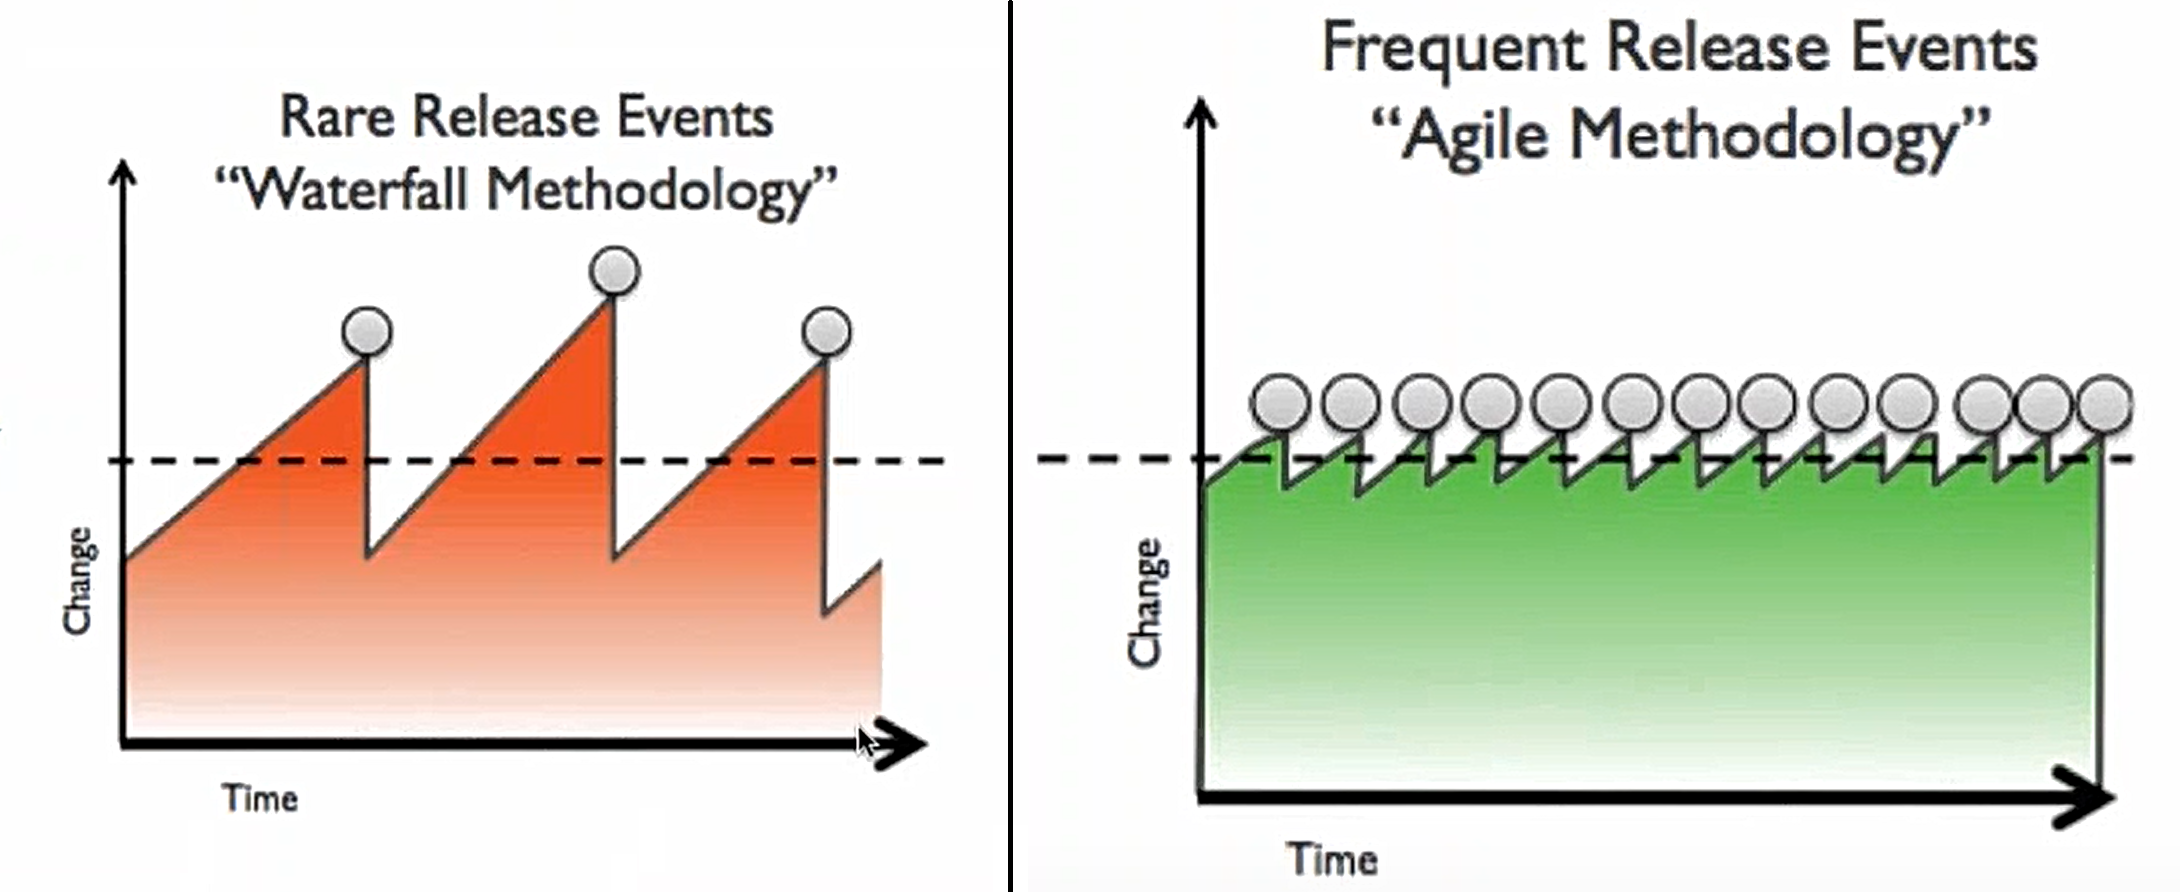
\includegraphics[width=\linewidth]{images/agile.png}
\caption{Agile vs Waterfall Methodology \cite{www-youtube-cf}}
\label{fig:agile}
\end{figure}

\TODO{Out of scope for the paper: This is too much on agile. Someone
  with a general CS background, which is your target audience, would
  know what agile is. You don't need the figure, and your summary of
  agile should be a couple sentences, not two paragraphs.}

\subsection{DevOps}
Devops is a set of practices for software testing and deployment which enables Agile development. Devops is a portmanteau of Development and Operations, signifying that the development and operations teams in a software company should coordinate to make quick releases possible. Typically after developing a software, developer sends it to the testing team, who then take another day or more to perform functional tests, get back with bugs. The developer has to fix them and send it back to the testing team. There is an inherent latency to this process that there are too many manual tasks involved. Devops kicks in here to set standards to automate testing and to ensure that production, QA and Development environments are in sync. It would also mean giving greater responsibility towards developers, and greater accesses \TE to environments for easy testing and development. With automated processes for testing, developers would get their feedback within minutes, and they can fix them without waiting for another team to respond. The final aspect of devops is to automate deployment. Once development and testing is done, there are software \GE to automatically deploy the software on a host of servers with the right configurations and connections, thus reducing manual effort and latency. 

\TODO{Scope: It's more reasonable to provide an explanation of devops
  than agile, but this is too long. Please try to condense to e.g. a
  couple sentences. You need to focus on PWS.}

\subsection{Platform as a service}
The concept of containers started gaining popularity considering the advantages of modularity in software development. Modularity implies that every piece of software is individual and self sufficient with capabilities to communicate with other modules. \TODO{Out of scope sentence. You don't need to explain what software modularity is.} Containers in software development serve the purpose of building modular software. A container will have the actual software along with all its dependencies and methods. \TODO{Paragraph should be shortened. Currently, only the last sentence tells the reader something they might not be familiar with (what a container is).}

Platform as a service (PaaS) or application platform as a service (aPaaS) is a category of cloud computing services that provides a platform allowing customers to develop, run, and manage applications without the complexity of building and maintaining the infrastructure typically associated with developing and launching an app \cite{www-paas-wiki}. PaaS providers generally provide a cloud environment to deploy the application on, the networks, servers, OS, storage, databases and other services to run applications. This removes the hassles of maintaining and running the servers and systems for an application from the developers, and also minimises the risk of server failures. 

\TODO{The second paragraph does a good job of summarizing PaaS. The first is mostly unnecessary. Please shorten the section.}

\subsection{Pivotal Web Services}
PWS is built based on an open source PaaS Cloud Foundry \TODO{Please explain what Cloud Foundry is.} along with some proprietary additions such as Pivotal's Developer Console, Billing Service and Marketplace \cite{www-pws-register}. PWS offers hosted cloud systems with a web interface for managing the environment, and a number of pre-provisioned services like relational databases and messaging queues \cite{www-pws-stackoverflow}. 

\section{Features of PWS}

PWS offers a lot of hassle free options to deploy and manage software \cite{www-pws-features}. 

\TODO{"hassle free" is subjective and more appropriate to advertisment.}

\subsection{Upload}
cf push \TODO{If you will include commands, please format as source code. However, including a command a specific command like this is too fine a detail for an overview paper like this. Please focus on the general process of using PWS rather than specific commands.} is a single command way to upload software developed on local to the cloud. The code is transformed into a running application on the cloud. The steps to follow for uploading an application with name <APP-NAME> is given in \cite{www-pws-push}.
\subsection{Stage}
Behind the scenes, the deployed application goes through staging scripts called buildpacks to create a ready-to-run droplet. \TODO{What is a droplet?} Buildpacks are software packets that provide framework and runtime support for applications, and they are provided along with PWS cloud. Buildpacks typically examine user-provided artifacts to determine what dependencies to download and how to configure applications to communicate with bound services. Cloud Foundry automatically detects which buildpack is required and installs it on the Diego cell where the application needs to run \cite{www-pws-buildpacks}. \TODO{This sounds very abstract. An example would help in understanding the process.}

\subsection{Distribute}
Deigo is the container management system for Cloud Foundry, which handles application scheduling and management. Each application VM has a Diego Cell that executes application start and stop actions locally, manages the VM’s containers, and reports app status and other data. Deigo Core has five main components, Brain, Cells, Database VMs, Access VMs, Consul \cite{www-pws-diego}.

\TODO{Listing the components of Deigo is unnecessary since this is not
  the focus of the paper and you don't mention them again.}

\subsection{Run}
Applications receive entry in a dynamic routing tier, which load balances traffic across all app instances. 

\section{Licensing}
Though Cloud Foundry is open source, it is not easy to maintain a cloud and setup the architecture by a developer. PWS is charges for the use of its services, with a monthly cost depending upon the memory of application instance and number of instances \cite{www-pws-pricing}. \TODO{You don't need to reference PWS' pricing. You need to explain how the license allows us to use the software.}

\section{Use Cases}
PWS can be used for a range of applications, from running websites to maintaining mobile applications. For example, if we need to host a website which accesses data, we can write the base code and deploy to PWS cloud.

\TODO{Your paper will benefit greatly if you add an actual use
  case. So far, your discussion has been very general, which makes
  understanding PWS' utility hard.}

\section{Conclusion}
PWS offers easy to use and hassle free \TODO{"easy to use" and "hassle free" are subjective} hosted cloud platform services, which offers a great alternative to AWS Elastic Beanstalk, Google cloud and Microsoft Azure. \TODO{This is the first time you've mentioned these. The conclusion is not a good place to introduce new platforms.}
Pivotal Web Services is one of the leading enterprise PaaS, powered by Cloud Foundry. \TODO{This sentence is subjective and doesn't convey and information.} It delivers a turnkey experience for scaling and updating PaaS on the private cloud, with no downtime. Pivotal Cloud Foundry enables developers to provision and bind web and mobile apps with leading \TODO{"leading" is subjective} platform and data services such as Jenkins, MongoDB, Hadoop, etc. on a unified platform. It empowers \TODO{"empowers" is a marketing term} businesses to deliver applications and update them with new features at a velocity and scale previously only available to Internet giants, allowing enterprises to innovate with disruptive speed \cite{www-pws-adv}.

\TODO{The conclusion as-is sounds like a press release or advertisment
  and should be rewritten.}

\section{Further Education}
Further learning about Pivotal is encouraged and informative materials can be found at the Pivotal homepage \cite{www-pws-agile}.

\section*{Acknowledgements}

The author thanks Professor Gregor Von Lazewski for providing us with the guidance and topics for the paper. The author also thanks the AIs of Big Data Class for providing the technical support.


% Bibliography

\bibliography{references}
 
\section*{Author Biographies}
\begingroup
\setlength\intextsep{0pt}
\begin{minipage}[t][3.2cm][t]{1.0\columnwidth} % Adjust height [3.2cm] as required for separation of bio photos.
{\bfseries Harshit Krishnakumar} is pursuing his MSc in Data Science from
Indiana University Bloomington
\end{minipage}
\endgroup

\end{document}
